\documentclass{article}
\usepackage{amsmath}
\usepackage{graphicx}
\usepackage{amsthm}
\usepackage{amssymb}
\usepackage[margin=2cm]{geometry}

\newcommand{\eqn}[1]{
  \begin{tabular}{|c|}
  \hline
  $#1$\\
  \hline
  \end{tabular}
}
\title{ILP-Based Synthesis for Sample Preparation
Applications on Digital Microfluidic Biochips}
\author{Abhimanyu}
\begin{document}

\maketitle

\section{Introduction}
This document describes a method to convert the information from a given application graph
and chip architecture into a system of linear inequations which can be given as an input 
to the ILP solver to obtain the the binding and scheduling result.

\section{Application Graph}
The application graph gives the information of the required chronological order of the 
operations. To show how to build up the inequations from the application graph, it would 
be best to use a graph as an example.\\

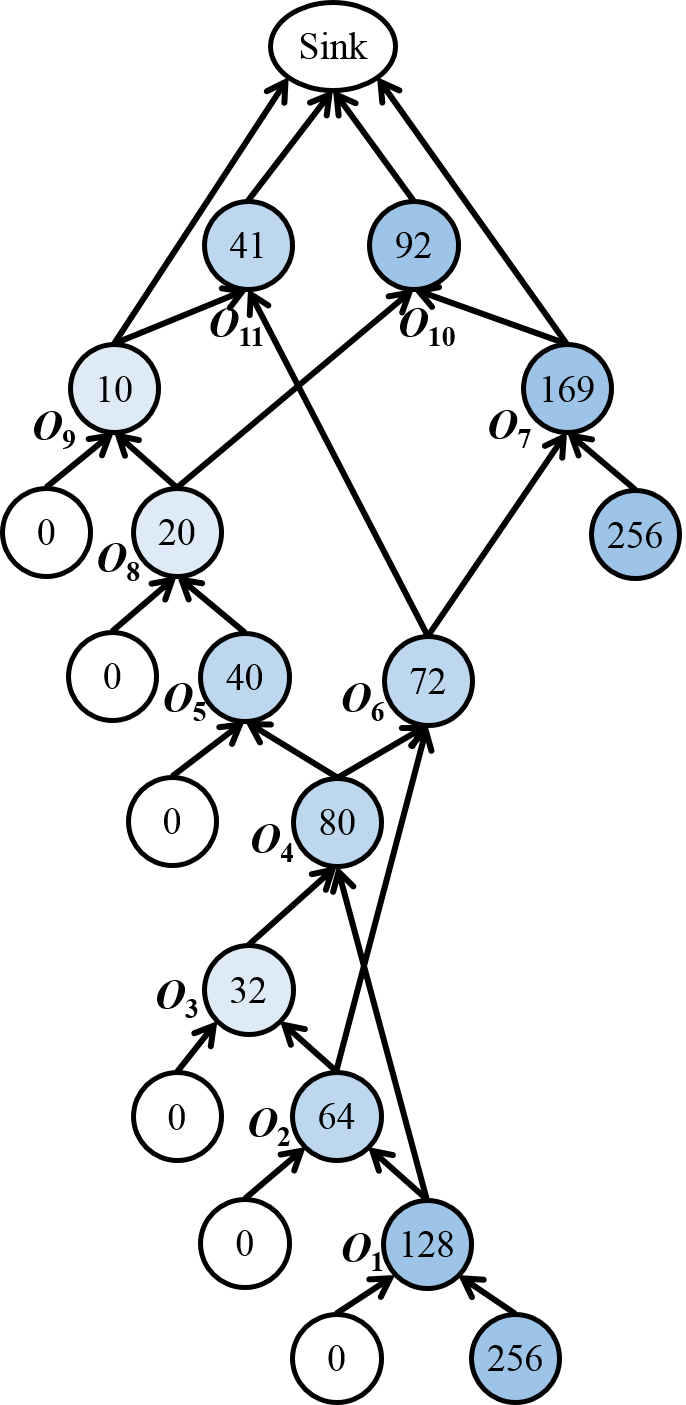
\includegraphics[width=0.5\textwidth, height=7cm]{a4.png}\\\\
Let \emph{$O_i$} represent the operation MIX i.\\ 
Let \emph{$s_i$} be the starting time step of operation $O_i$. \\
Let \emph{T($O_i$}) be the time required to perform the operation $O_i$, 
it will be given in the Chip Architecture, but since only one type of
operation i.e. MIX is being done, T($O_i$) will be the same $\forall$ i.\\
Let \emph{n} be the total number of mixing operations.\\
\begin{center}
\begin{tabular}{|c|c|}  
\hline
Operation & Inequation\\
\hline
$O_1$ & $s_1\geq 0$\\
$O_2$ & $s_2\geq s_1 + T(O_1)$\\
$O_3$ & $s_3\geq s_1 + T(O_1)$\\
$O_4$ & $s_4\geq s_2 + T(O_2)$\\
$O_5$ & $s_5\geq s_3 + T(O_3)$\\
$O_6$ & $s_6\geq s_4 + T(O_4)$\\
$O_7$ & $s_7\geq s_5 + T(O_5)$\\
\hline
\end{tabular}
\end{center}

\noindent
 We create a dummy variable $s_8$ such that $s_8 \geq s_6, s_8 \geq s_7$\\
\textbf{\emph{Objective}: Minimize $s_8$}

\section{Scheduling result}
\emph{Note}: Time steps start from 0. \emph{$T_{MAX}$} is the highest value the time step 
can take. We can define \emph{$T_{MAX}$} to be the time it would take to finish the complete
application doing only 1 operation at a time. It is just a very loose upper bound.\\  
\subsection{Mixing}
We declare a class of binary variables \{$X_{it}$ $\forall i$, $\forall t$\} such that: \\

\begin{equation*}
  X_{it} = \begin{cases}
  1  &  \text{if }O_i \text{ is running at time step t} \\
  0  &  \text{if }O_i \text{ is \emph{not} running at time step t}
  \end{cases}
\end{equation*}

\subsubsection{Formulation}
For a given i and t:\\\\
if ($s _i \leq t < s_i + T(O_i)$) \\
\indent $X_{it} = 1$\\
else\\
\indent $X_{it} = 0$\\
\\\noindent \textbf{Inequations} for the above if-else-condition.

\begin{center}
\begin{tabular}{|c|}
\hline
$t-s_i \geq T_{MAX}*(X_{it}-1)$\\
$s_i + T(O_i) - t > T_{MAX}*(X_{it}-1)$\\
$\sum\limits_{t=0}^{T_{MAX}}X_{it}=T(O_i)$\\
\hline
\end{tabular}
\end{center}

\subsection{Storage}
Let E be the set of all edges of the graph which start and terminate on a MIX node and $\|E\|=n_e$.We declare a class of binary variables \{$Y_{et}$ $\forall e$, $\forall t$\} such that: \\

\begin{equation*}
  Y_{et} = \begin{cases}
  1  &  \text{if Droplet of egde e is being stored at time step t} \\
  0  &  \text{if Droplet of egde e is  not being stored at time step t} \\
  \end{cases}
\end{equation*}

\subsubsection{Formulation}
For a given e (where e is the edge between i and j) and t:\\\\
if ($s _i + T(O_i) \leq t < s_j$) \\
\indent $Y_{et} = 1$\\
else\\
\indent $Y_{et} = 0$\\
\\\noindent \textbf{Inequations} for the above if-else-condition.

\begin{center}
\begin{tabular}{|c|}
\hline
$t-(s_i + T(O_i)) \geq T_{MAX}*(Y_{et}-1)$\\
$s_j - t > T_{MAX}*(Y_{et}-1)$\\
$\sum\limits_{t=0}^{T_{MAX}}Y_{et}=s_j-(s_i + T(O_i))$\\
\hline
\end{tabular}
\end{center}

\section{Chip Architecture Constraints}
We have $n_m$ modules available. In general, depending on the size of the module, it can be used either as mixer or a storage for $n_r$ droplets. Here, we will be considering the the special case of $n_r = 1$ . $\therefore$ we can have a total of  $n_m$ mixing and storage operations atmost. \\
We get the following constraint from this:\\
\\
\begin{tabular}{|c|}
\hline
$\forall t \sum\limits_{i=1}^n X_{it} + \sum\limits_{e=1}^E Y_{et}\leq n_m$\\  
\hline
\end{tabular}
\\
\\
\noindent where \emph{n} is the number of mixing operations.


\subsection{Binding result for Mixing}
Let \{$M_{pi}$ $\forall p$, $\forall i$\} be a class of binary variables such that:\\

\begin{equation*}
  M_{pi} = \begin{cases}
  1  &  \text{if }O_i \text{ is bound to Mixer p} \\
  0  &  \text{if }O_i \text{ is \emph{not} bound to Mixer p}
  \end{cases}
\end{equation*}

\begin{itemize}

\item To ensure that an operation remains bound to the
same module throughout the time it is being executed, we have 
the following inequation:\\\\
\eqn{\sum\limits_{p=1}^{n_m}M_{pi}=1}\\

\item If two operations i, j are bound to the same module p, then 
there can't be a time step t when both of them are running simultaneously.\\
\\
For all mixing operations i, j and $i\neq j$ \\if($M_{pi}=M_{pj}=1$)\\
\indent $\forall t$ $X_{it}+ X_{jt} < 2$\\
\\
The in-equations corresponding to the above are as follows:\\ 
\begin{tabular}{|c|}
\hline
$X_{it}+X_{jt}\geq M_{pi}+M_{pj}-2$\\
$X_{it}+X_{jt}\leq 3-(M_{pi}+M_{pj})$\\
\hline
\end{tabular}
\end{itemize}

\subsection{Binding result for Storage}
Let \{$R_{pe}$ $\forall p$, $\forall e$\} be a class of binary variables such that:\\

\begin{equation*}
  R_{pe} = \begin{cases}
  1  &  \text{if droplet of edge e is bound to Mixer p} \\
  0  &  \text{if droplet of edge e is \emph{not} bound to Mixer p}
  \end{cases}
\end{equation*}

\begin{itemize}

\item To ensure that a droplet remains bound to the
same module throughout the time it is being executed, we have 
the following inequation:\\\\
\eqn{\forall e \sum\limits_{p=1}^{n_m}R_{pe} \leq 1}\\

\item If two edges i, j are bound to the same module p, then 
there can't be a time step t when both of them are being stored.\\
\\
For all edges i, j and $i\neq j$ \\if($R_{pi}=R_{pj}=1$)\\
\indent $\forall t$ $Y_{it}+ Y_{jt} < 2$\\
\\
The inequations corresponding to the above are as follows:\\ 
\begin{tabular}{|c|}
\hline
$Y_{it}+Y_{jt}\geq R_{pi}+R_{pj}-2$\\
$Y_{it}+Y_{jt}\leq 3-(R_{pi}+R_{pj})$\\
\hline
\end{tabular}
\end{itemize}
\subsection{Additional Constraint}
We also need to ensure that a module should not be used as both a reservoir and mixer at the same time. We have the following in-equation for this.\\
\\
\eqn{\forall p, \forall t \sum\limits_{i=1}^n M_{pi}*X_{it} + \sum\limits_{e=1}^E R_{pe}*Y_{et} < 2}\\\\

\emph{Interpretation} For a given module p, the first summation is 1 at the time step when an operation bound to this module is running at that time step. The in-equation prevents the module from storing any droplet at that time. Similarly, the second summation is 1 at the time step when a droplet bound to this module is being stored. The in-equation prevents the module from any mixing operation.

\noindent We can use the following methodology for AND formulation.\\\\
\begin{tabular}{|c|}
\hline
Inequations for $L_{pit}=M_{pi}*X_{it}$\\
\hline
$L_{pit} \geq M_{pi} + X_{it} - 1$\\
$L_{pit} \leq M_{pi} + X_{it}$\\
$L_{pit} \leq 1-(M_{pi} - X_{it})$\\
$L_{pit} \leq 1-(X_{it} - M_{pi})$\\
\hline 
\end{tabular}
\\\\\\
\begin{tabular}{|c|}
\hline
Inequations for $G_{pet}=R_{pe}*Y_{et}$\\
\hline
$G_{pet} \geq R_{pe} + Y_{et} - 1$\\
$G_{pet} \leq R_{pe} + Y_{et}$\\
$G_{pet} \leq 1-(R_{pe} - Y_{et})$\\
$G_{pet} \leq 1-(Y_{et} - R_{pe})$\\
\hline 
\end{tabular}
 

\end{document}
